\documentclass[11pt,letterpaper]{article}
\usepackage[T1]{fontenc}
\usepackage{amsmath}
\usepackage{amsfonts}
\usepackage{amssymb}
\usepackage{graphicx}

\usepackage[charter]{mathdesign}
\usepackage{fullpage}
\pagestyle{empty}

\NeedsTeXFormat{LaTeX2e}
\ProvidesClass{fncextra}[2017/01/24 LaTeX Class For FNC extra materials]

\LoadClass{article}
\DeclareOption*{\PassOptionsToClass{\CurrentOption}{article}}
\ProcessOptions\relax

\RequirePackage{amsmath}
\RequirePackage[headings]{fullpage}
\RequirePackage[utopia]{mathdesign}
\RequirePackage{bm}
\RequirePackage{url}

\lstset{style=Matlab-editor,basicstyle=\ttfamily}
\definecolor{lightgray}{gray}{0.5}

\newcommand{\nat}{\mathbb{N}}          % Natural numbers
\newcommand{\integer}{\mathbb{Z}}      % Integers
\newcommand{\real}{ {\mathbb{R}} }     % Reals
\newcommand{\float}{ {\mathbb{F}} }     % Reals
\newcommand{\rmn}[2]{ \mathbb{R}^{#1\times#2} }     % Reals
\newcommand{\complex}{ {\mathbb{C}} }  % Complex
\newcommand{\macheps}{\ensuremath \varepsilon_{\text{mach}}}

\renewcommand{\Re}{\operatorname{Re}}
\renewcommand{\Im}{\operatorname{Im}}

% Boldface vectors
\newcommand{\bff}{\bm{f}}
\newcommand{\bfF}{\bm{F}}
\newcommand{\bfw}{\bm{w}}
\newcommand{\bfv}{\bm{v}}
\newcommand{\bfe}{\bm{e}}
\newcommand{\bfc}{\bm{c}}
\newcommand{\bfp}{\bm{p}}
\newcommand{\bfq}{\bm{q}}
\newcommand{\bfr}{\bm{r}}
\newcommand{\bfs}{\bm{s}}
\newcommand{\bfu}{\bm{u}}
\newcommand{\bfb}{\bm{b}}
\newcommand{\bfx}{\bm{x}}
\newcommand{\bfy}{\bm{y}}
\newcommand{\bfg}{\bm{g}}
\newcommand{\bfh}{\bm{h}}
\newcommand{\bfz}{\bm{z}}
\newcommand{\bfa}{\bm{a}}
\newcommand{\bft}{\bm{t}}
\newcommand{\bfd}{\bm{d}}
\newcommand{\bfalpha}{\bm{\alpha}}
\newcommand{\bfeps}{\bm{\varepsilon}}
\newcommand{\bfdelta}{\bm{\delta}}
\newcommand{\bfzero}{\bm{0}}
\newcommand{\eye}[1]{\bfe_{#1}}

% Boldface matrix
\newcommand{\m}[1]{\bm{#1}}
\newcommand{\mA}{\m{A}}
\newcommand{\mL}{\m{L}}
\newcommand{\mF}{\m{F}}
\newcommand{\mU}{\m{U}}
\newcommand{\mJ}{\m{J}}
\newcommand{\mP}{\m{P}}
\newcommand{\mQ}{\m{Q}}
\newcommand{\mR}{\m{R}}
\newcommand{\mD}{\m{D}}
\newcommand{\mS}{\m{S}}
\newcommand{\mB}{\m{B}}
\newcommand{\mC}{\m{C}}
\newcommand{\mE}{\m{E}}
\newcommand{\mG}{\m{G}}
\newcommand{\mH}{\m{H}}
\newcommand{\mV}{\m{V}}
\newcommand{\mW}{\m{W}}
\newcommand{\mX}{\m{X}}
\newcommand{\mZ}{\m{Z}}
\newcommand{\mK}{\m{K}}
\newcommand{\mM}{\m{M}}

\newcommand{\meye}{\m{I}}

\newcommand{\ee}[1]{\times 10^{#1}}
\newcommand{\jac}[2]{\frac{\bfd \bm{#1}}{\bfd \bm{#2}}}
\newcommand{\diag}{\operatorname{diag}}
\newcommand{\fl}{\operatorname{fl}}
\newcommand{\circop}[1]{\makebox[0pt][l]{$\bigcirc$}\hspace{1pt}#1}
\newcommand{\myvec}{\operatorname{vec}}
\newcommand{\unvec}{\operatorname{unvec}}
\newcommand{\kron}[2]{#1 \otimes #2}
\newcommand{\mtx}{\operatorname{mtx}}
\newcommand{\fun}{\operatorname{fun}}


\begin{document}
	
\begin{center}
  \bf 
  Project: Getting nervous?
\end{center}
	
There are many important \textit{activator--inhibitor} phenomena, in which two components of a system essentially compete to pull it in different directions, leading to oscillatory behavior. A classic example is the \emph{FitzHugh--Nagumo} model of a neuron: \begin{equation}
  \label{eq:fh}
  \begin{split}
    \frac{dv}{dt} &= v(a-v)(v-1) - w + \beta, \\
    \frac{dw}{dt} &= b v - c w,
  \end{split}
\end{equation}
where $0<a<1$, and $b$, $c$, and $\beta$ are positive constants. In physically realistic models, $v$ stands for an activation potential, and the peaks in $v$ correspond to ``firing'' a signal. The parameter $\beta$ is analogous to an external current enhancing the growth of $v$, and it affects the period of the oscillations.

A steady state of the ODE occurs when $v'(t)=w'(t)=0$. These conditions imply a nonlinear system of two equations for the two variables $v$ and $w$. 

\hfill \rule{4in}{1pt} \hspace*{\fill}\\

\noindent \textbf{Objective 1 (20\% of the grade).} Let $a=1$ and $c=4$. Starting from the values $v=1$, $w=0$, calculate by hand the symbolic result of taking one Newton step to solve the nonlinear system. Your answer will be in terms of $b$ and $\beta$. (\emph{Note:} It would be trivial to solve for $w=bv/c$, eliminate $w$, and obtain a single equation in only $v$. But for the purposes of this problem, leave it as two equations in two variables.)

For this objective, submit the following:
\begin{itemize}
\item A PDF (typeset nicely or scanned from a neatly written document)
  \texttt{objective1.pdf} 
  that shows the function value and Jacobian matrix at the given
  initial vector, and the values of $v$ and $w$ after the Newton step. 
\end{itemize}

\hfill \rule{4in}{1pt} \hspace*{\fill}\\

You can see solutions of the model as an initial-value problem for two different values of $\beta$ in Figure~1, for which
\begin{equation}
  \label{eq:param}
  a=0.25,\quad b=c=0.02, \quad   v(0)=0.1,\quad w(0)=0.
\end{equation}


\begin{figure}[bt]
  \centering
  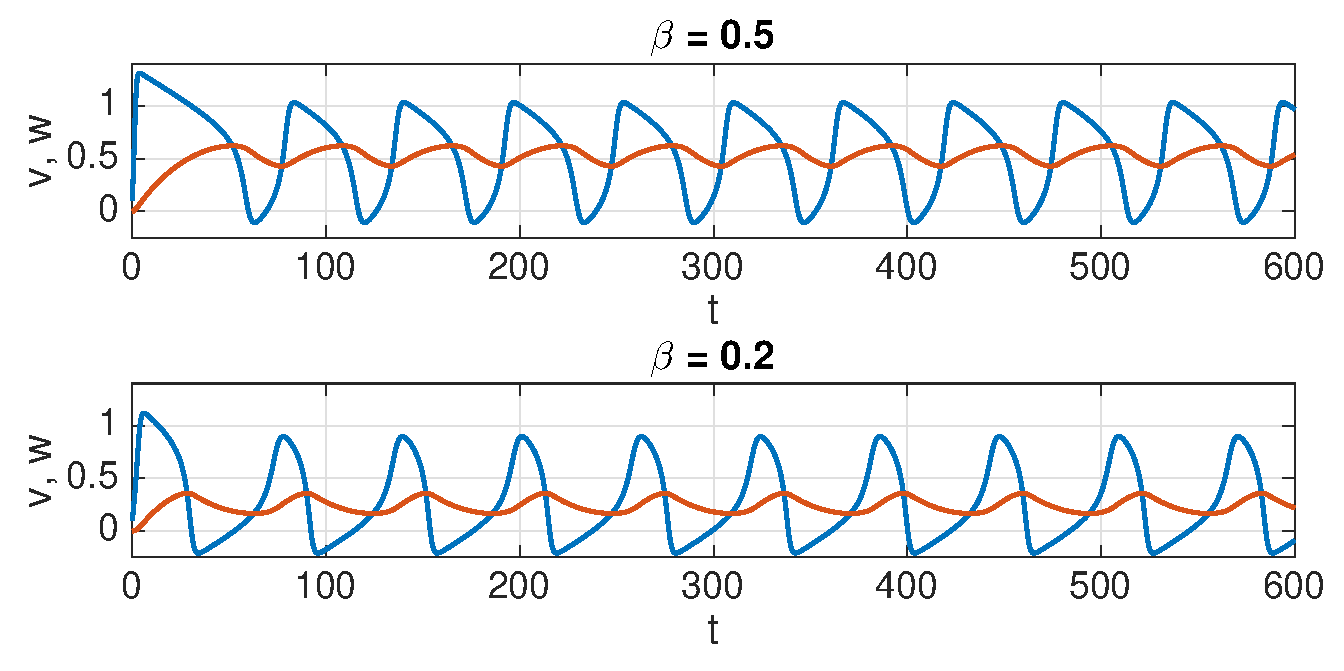
\includegraphics[width=\textwidth]{FHexample}
  \caption{Solutions of the system~(1) using the values in~\eqref{eq:param} and two different values of $\beta$.}
  \label{fig:fh}
\end{figure}

\hfill \rule{4in}{1pt} \hspace*{\fill}\\

\noindent \textbf{Objective 2 (20\% of the grade).}  Recreate Figure~1 using the single-neuron model~(1) and the parameters in~\eqref{eq:param}. (You do not need to worry about details such as line width, font size, axes size, etc.) Then, on one other graph, plot the two solutions in the $(v,w)$ phase plane.

For this objective, submit the following:
\begin{itemize}
\item A file \texttt{figure1.pdf}, which is your recreation of
  Figure~1.
\item A file \texttt{phaseplane.pdf}, which is your phase plane plot. 
\item A file called \texttt{objective2.m} which can be executed to
  produce the graphs as separate MATLAB figures.
\item \textit{All} other M-files needed for successful execution.
\end{itemize}

\hfill \rule{4in}{1pt} \hspace*{\fill}\\

From Figure~1 (top half) we can estimate the period of oscillation when $\beta=0.5$. Imagine drawing a horizontal line in Figure~1 with $v=1/2$. For each oscillation, this line makes two intersections with the graph of $v(t)$ in blue: one when $v$ is increasing, and another when $v$ is decreasing. Hence we can define one period of the oscillation as the time between two similar kinds of intersections (i.e., both increasing or both decreasing). 

We can extend the idea to get much more precision than a simple graphical estimate allows. Note that 
whichever kind of intersection we pick (increasing or decreasing), there is a particular value of $w$ associated with it. So we can define the period $T$ via the conditions $v(0)=v(T)=1/2$, $w(0)=w(T)$. If we let the initial conditions be $v(0)=1/2$, $w(0)=\gamma$, then we can solve the model over $[0,T]$ and check the equations $v(T)=1/2$, $w(T)=\gamma$, which will be valid only when $\gamma$ and $T$ are chosen correctly. In other words, we have defined a system of two equations $\bff\,(\bfx)=\bfzero$ for the unknowns $x_1 = \gamma$ and $x_2 = T$. 

\hfill \rule{4in}{1pt} \hspace*{\fill}\\

\noindent \textbf{Objective 3 (30\% of the grade).} Find the oscillation period with $a=0.25$, $b=c=0.02$, and $\beta=0.5$ by using \texttt{levenberg} from the text on the system of equations described above. As always, you must provide \texttt{levenberg} with the function $\bff(\bfx)$. 
%\footnote{The big picture is that you write a
%  script that calls \texttt{levenberg}, which must use a function
%  that you write for~\eqref{eq:period}, which calls an \texttt{ode}
%  solver, which must call on another function that you write
%  for~\eqref{eq:fh}.} 
You can find a good starting value for \texttt{levenberg} using the graph you made for Objective 2.

For this objective, submit the following:
\begin{itemize}
\item A PDF file called \texttt{period.pdf} showing the sequence of estimates of $T$ produced by \texttt{levenberg}.  
\item A file called \texttt{objective4.m} which can be executed to produce the same sequence of estimates.
\item \textit{All} other M-files needed for successful execution.
\end{itemize}

\hfill \rule{4in}{1pt} \hspace*{\fill}\\

Some oscillators exhibit an interesting phenomenon of synchronization. If the oscillators are coupled together, even weakly, they can adjust their individual natural frequencies to oscillate together. This can occur with pendulums, fireflies\footnote{See
  https://youtu.be/a-Vy7NZTGos, for example.}, and neurons. To extend
our equations to two neurons, we use
% \begin{equation}
%   \label{eq:fhsys}
%   \begin{split}
%     \frac{dv_i}{dt} &= v_i(a-v_i)(v_i-1) - w_i + \beta_i + \alpha
%     \sum_{\substack{j=1\\j\neq i}}^N v_j, \qquad i=1,\ldots,N,\\
%     \frac{dw_i}{dt} &= b v_i - c w_i,
%   \end{split}
% \end{equation}
\begin{equation}
  \label{eq:fhsys}
  \begin{split}
    \frac{dv_1}{dt} &= v_1(a-v_1)(v_1-1) - w_1 + \beta_1 + \alpha v_2,\\
    \frac{dv_2}{dt} &= v_2(a-v_2)(v_2-1) - w_2 + \beta_2 + \alpha v_1,\\
    \frac{dw_1}{dt} &= b v_1 - c w_1,\\
    \frac{dw_2}{dt} &= b v_2 - c w_2,
  \end{split}
\end{equation}
Here, the excitation of $v_i$ occurs in response to the 
firing of the other neuron, with a strength expressed as $\alpha >
0$. Larger values of $\alpha$ mean stronger coupling.


\hfill \rule{4in}{1pt} \hspace*{\fill}\\

\noindent \textbf{Objective 4 (30\% of the grade).} Implement the model~\eqref{eq:fhsys}, using $\beta_1=0.5$, $\beta_2=0.2$, $v_1(0)=v_2(0)=0.25$, $w_1(0)=w_2(0)=0$, and $a$, $b$, and $c$ as given in~\eqref{eq:param}. Make a $2\times 1$ subplot grid. In the top axes plot $v_1(t)$ and $v_2(t)$ over $0\le t \le 1000$ for $\alpha = 0.002$, and in the bottom axes make the same plot for the solution with $\alpha=0.05$. It should be clear that the top pair never synchronize while the bottom pair quickly reach the same frequency.

For this objective, submit the following:
\begin{itemize}
\item A file \texttt{sync.pdf} showing the graph described above.
\item A file called \texttt{objective5.m} which can be executed to
  produce the graph as a MATLAB figure.
\item \textit{All} other M-files needed for successful execution.
\end{itemize}


\vfill

\begin{center}
  \includegraphics[height=2in]{neuronthinking}
\end{center}

\end{document}

